% setup the document and include packages
\documentclass{article}[12pt]
\usepackage{graphicx}
\usepackage{amsmath}
\usepackage{amssymb}
\usepackage{cancel}
\usepackage{ntheorem}
\usepackage{algorithm2e}
\usepackage{float}
\usepackage{caption}
\usepackage{fancyvrb}
\usepackage[dvipsnames]{xcolor}
\usepackage[section]{placeins}
\usepackage[toc,page]{appendix}
\usepackage{hyperref}
\usepackage{subfig}

%set stuff for syntax highlighting
%\usepackage{fontspec}
%\usepackage{minted}
%\setsansfont{Calibri}
%\setmonofont{Consolas}
\usepackage{hyperref}
\hypersetup{
    colorlinks=true,
    linkcolor=blue,
    filecolor=magenta,      
    urlcolor=cyan,
}
\urlstyle{same}

\makeatletter
\def\BState{\State\hskip-\ALG@thistlm}
\makeatother

% define Continue for algorithms
\SetKw{Continue}{continue}

% redefine QED symbol
\renewcommand{\qedsymbol}{\rule{0.7em}{0.7em}}

% define lemma and result theorem-styled sections
\newtheorem{lemma}{Lemma}[section]
\newtheorem{result}{Result}[section]

% setup paths for images
\graphicspath{ {../scripts/plots/} }

% Don't print the semicolon in algorithms
\DontPrintSemicolon

% define the title that will be used in the report
\title{CS 440 M4P4\\ Section Q4 \\ 4 Credits}
\author{
Luke Pitstick \\ pitstck2@illinois.edu
}
\date{} % don't set a date because we don't need this shit


% start the document
\begin{document}
   
   % create the title page 
   \maketitle
   \begin{abstract}
abstract
   \end{abstract}
   \newpage

   
   % start section covering work on Part 1.1
   \section{Digit Classification using Discriminative Machine Learning Methods} \label{sec:one}
   
   \subsection{Digit Classification with Perceptrons}
   
   First digit classification is done with a multi-class perceptron. Each pixel is considered a feature with 784 in total. First the program reads all the digits into the system in a binary format. It then passes through all the training examples and obtains a result $y_c = w \cdot x$ where $y_c$ is the result for a single class and $w\cdot x$ is the dot product of the weight and feature vectors. Then the maximum result is selected ass the temporary guess for that round. If correct, the weights are left unchanged. If incorrect the expected class is updated as $w_{cc} = w_{cc} + \alpha x$ and the guessed class as $w_{cg} = w_{cg} - \alpha x$. Alpha is the learning rate which decays over time. This process is repeated multiple times (epochs) over the same training set.
   
   Once the weights have been trained the same guessing procedure is done just once on each example in the testing set, and the results are recorded. The best settings that were selected were with bias, initial weights as random, random training order, and inverse decay. The selection of these is discussed later. These were then tested over a range of epochs to see the effect on overall accuracy. Figure 1 contains these results.
   
      \begin{table}[ht]
   	\centering
   	\begin{tabular}{l | c | c}
   		\hline
   		 Epochs  & Accuracy & Runtime (s)\\
   		\hline \hline \hline
   		1 & 76.9\% & 0.4\\
   		2 & 71.7\% &0.6\\
   		3 & 82.2\% &0.8\\
   		4 & 80.3\% &1.0\\
   		5 & 82.7\% &1.4\\
   		10 & 83.1\% &3.9\\
   		15 & 82.5\% &3.3\\
   		20 & 80.9\% &4.2\\
   		30 & 82.4\% &5.8\\
   		40 & 82.1\% &8.5\\
   		50 & 82.9\% &10.9\\
   		100 & 82.3\% &21.1\\
   		200 & 81.9\% &42.4\\
   		500 & 82.4\% &102.9\\
   		\hline
   	\end{tabular}
   	\caption{Classification Accuracy by Number of Epochs} \label{tab:digacc}
   \end{table}
   
   We can see that accuracy improves early on with the increase in number of epochs. We see a leveling off after 30 epochs around the accuracy of 82\%. The highest values being at 10 epochs is likely due to a random variation in the weights that made it get some lucky guesses. We decided to use 50 epochs for all further test because it is after the leveling point with good results. This also gives us the confusion  in figure 2 which shows how often digits from the rows on the left were identified as the classes from the row on the top.
   
   Runtime scaled linearly to epochs as expected. It took roughly epochs/5 in seconds to run. 

   
      \begin{figure}[!htb]
   	\centering
   	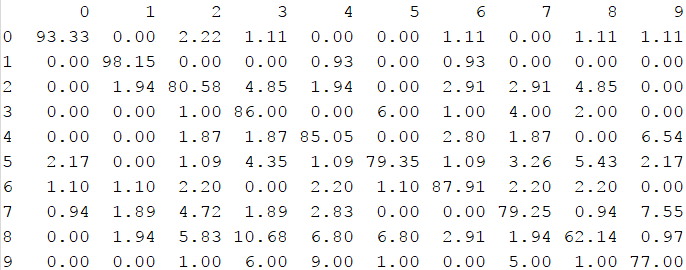
\includegraphics[scale=0.7]{confusion.png}
   	\caption{Perceptron Confusion Matrix}
   	\label{fig:cm11}
   \end{figure}
   
   As mentioned above, the overall accuracy obtained with optimal settings is 82.9\%. The bias was implemented by having a feature dimension that was a constant 1 for all images. This helps account for the overall frequency that a class appears. Without a bias accuracy is 82.5\%, so using bias performs better. The inital weights could be set to either 0 or a random range between -10 and 10. When set to 0 overall accuracy was 81.5\%, so random weights were used. Before each epoch the training examples could remain in a static order, or be shuffeled each time. Without shuffling the accuracy is 81.7\%, so shuffling is used for the best results. Finally the best decay function found was $\alpha=epochs/(epochs+t)$ where $t$ is the current epoch. This is an inverse decay. We also tested exponential decay $\alpha = e^{-t/epochs}$ with an accuracy of 81.9\%, and linear decay $\alpha = (-t/epochs)+1$ with an accuracy of 81.5\%.
  
   The single pixel Naive Bayes approach gave an overall accuracy of 77.5\%, so clearly the perceptron approach was much more accurate. The combinations with the highest confusion rates were nearly the same. The top 3 for both approaches are (8,3), (7,9), (4,9). But the Naive Bayes had (5,3) in the top four, while the perceptron had (3,5) instead. The perceptron also did better for each individual accuracy, except for 9's where Naive Bayes outperformed it. These previous results are in Figure 2.
   
    \begin{figure}[!htb]
   	\centering
   	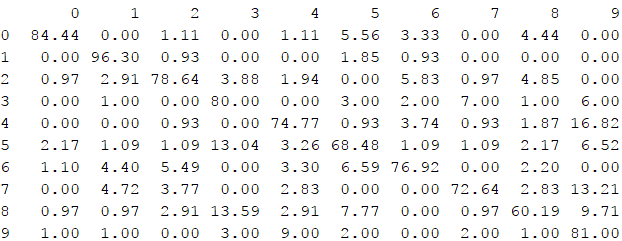
\includegraphics[scale=0.5]{confusion_nb.png}
   	\caption{Naive Bayes Confusion Matrix}
   	\label{fig:cm21}
   \end{figure}
   
   \newpage
   
  \subsection{Digit Classification with Nearest Neighbor}

  We performed the same image classification but using the k-nearest neighbors approach. This approach uses a distance function to find the k nearest training examples, and is classified as the most frequent one. My distance function is simply $d=abs(FA_{11} - FB_{11}) + abs(FA_{11} - FB_{11}) + ... + abs(FA_{11} - FB_{11})$. This is the sum of the absolute values of the differences between the features at each  index on each image.
  
        \begin{table}[ht]
   	\centering
   	\begin{tabular}{l | c | c}
   		\hline
   		 k  & Accuracy & Runtime (s)\\
   		\hline \hline \hline
   		1 & 90.2\% & 22.2\\
   		2 & 89.3\% & 22.2\\
   		3 & 89.0\% & 21.0\\
   		4 & 89.6\% &21.4\\
   		5 & 90.1\% & 22.1\\
   		10 & 88.8\% & 22.2\\
   		20 & 88.8\% & 22.2\\
   		50 & 88.6\% & 22.3\\
   		100 & 88.2\% &22.5\\
   		500 & 86.6\% & 25.9\\
   		\hline
   	\end{tabular}
   	\caption{Classification Accuracy by Number of Epochs} \label{tab:digack}
   \end{table}
   
   We see a slow decline in accuracy as k increases. The best overall accuracy is with k=1 of 90.2\%. The confusion matrix of this result is in Figure 3.
   
   The change in runtime is small, it increases it by .1s (less than 1\%) for even the larger k=100. It is a bit more significant at 3s for k=500, but that is only 15\% for a k which considers 1/10 of all entries as neighbors.  This is because k only influences the runtime when adding to and checking the k nearest neighbors. Adding doesn't happen too often once a few good values have been found. And selecting from it is just an O(k) operation. The bulk of computation time is spent comparing each test image to every single training image.
   
       \begin{figure}[!htb]
   	\centering
   	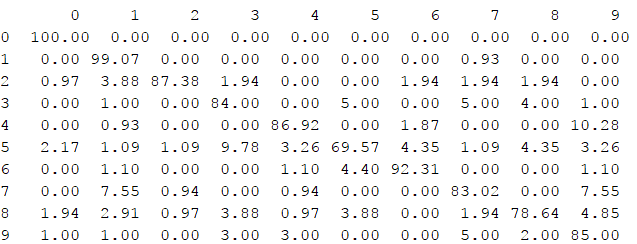
\includegraphics[scale=0.9]{confusion_knn.png}
   	\caption{KNN Confusion Matrix}
   	\label{fig:cm31}
   \end{figure}
   
   Performance was better than both the perceptron and the Naive Bayes implementations. However, we had different high confusion rates for this approach. KNN had trouble with similar pairs (5,3),(4,9), (7,9) and (3,5).

\end{document}